	%-=-=-=-=-=-=-=-=-=-=-=-=-=-=-=-=-=-=-=-=-=-=-=-=
%
%        LOADING DOCUMENT
%
%-=-=-=-=-=-=-=-=-=-=-=-=-=-=-=-=-=-=-=-=-=-=-=-=

\documentclass[newPxFont,pagenumber]{beamer}
\usetheme{sthlm}
%\usecolortheme{sthlmv42}

%-=-=-=-=-=-=-=-=-=-=-=-=-=-=-=-=-=-=-=-=-=-=-=-=
%        LOADING PACKAGES
%-=-=-=-=-=-=-=-=-=-=-=-=-=-=-=-=-=-=-=-=-=-=-=-=
\usepackage[utf8]{inputenc}
\usepackage[frenchb]{babel}
\usepackage[normalem]{ulem}
\usepackage{caption}
\captionsetup{font=scriptsize}
%\usepackage[font=footnotesize]{subcaption}
% in preamble
\usepackage{eurosym}
\usepackage{chronology}
\usepackage{pgf}
\usepackage{tikz}
\usetikzlibrary{arrows,automata}
\usepackage{array,multirow}
\usepackage{nameref}
\makeatletter
\newcommand*{\currentname}{\@currentlabelname}
\makeatother

\graphicspath{ {fig/} }

\usepackage[linesnumbered,ruled,vlined]{algorithm2e}
% add page number
%\usepackage[defaultsans]{cantarell}

\newcommand{\p}{\mathbb{P}}

\setbeamerfont{title}{series=\upshape}
\setbeamertemplate{footline}{\hfill\footnotesize\insertframenumber\hskip3pt\null\vskip3pt}

\newcommand{\argmax}{\mathop{\mathrm{argmax}}\limits}
\renewcommand{\max}{\mathop{\mathrm{max}}\limits}

\renewcommand{\event}[3][e]{%
  \pgfmathsetlength\xstop{(#2-\theyearstart)*\unit}%
  \ifx #1e%
    \draw[fill=black,draw=none,opacity=0.5]%
      (\xstop, 0) circle (.2\unit)%
      node[opacity=1,rotate=45,right=.2\unit] {#3};%
  \else%
    \pgfmathsetlength\xstart{(#1-\theyearstart)*\unit}%
    \draw[fill=black,draw=none,opacity=0.5,rounded corners=.1\unit]%
      (\xstart,-.1\unit) rectangle%
      node[opacity=1,rotate=45,right=.2\unit] {#3} (\xstop,.1\unit);%
  \fi}%

\addto\captionsfrench{%
\renewcommand{\figurename}{\scriptsize {\scshape Figure}}
\renewcommand{\tablename}{\scriptsize {\scshape Table}}
}

%-=-=-=-=-=-=-=-=-=-=-=-=-=-=-=-=-=-=-=-=-=-=-=-=
%        BEAMER OPTIONS
%-=-=-=-=-=-=-=-=-=-=-=-=-=-=-=-=-=-=-=-=-=-=-=-=

%\setbeameroption{show notes}
\setbeamersize{text margin left=5pt,text margin right=5pt}

%-=-=-=-=-=-=-=-=-=-=-=-=-=-=-=-=-=-=-=-=-=-=-=-=
%
%	PRESENTATION INFORMATION
%
%-=-=-=-=-=-=-=-=-=-=-=-=-=-=-=-=-=-=-=-=-=-=-=-=

\title{\normalsize Analyse sémantique d'un corpus exhaustif de décisions jurisprudentielles 
%p l'élaboration d'un modèle prédictif du risque judiciaire     
}
\subtitle{\scriptsize Comité de suivi individuel -- \textit{15 juin 2018}}
%\date{\small{\jobname}}
\date{\scriptsize Début de thèse: 15 Décembre 2015}
\author{\normalsize Gildas Tagny Ngompé}
\institute{\scriptsize \textbf{Direction de thèse:} \begin{itemize}
\item Jacky Montmain (École des mines d'Alès, LGI2P)
\item Stéphane Mussard (Université de Nîmes, CHROME)
\end{itemize}
\textbf{Encadrement de proximité:} \begin{itemize}
\item Sébastien Harispe (Ecole des Mines d'Alès, LGI2P)
\item Guillaume Zambrano (Université de Nîmes, CHROME)
\end{itemize}}

\hypersetup{
pdfauthor = {\author{}: tagnyngompe@gmail.com},
pdfsubject = {},
pdfkeywords = {},
pdfmoddate= {D:\pdfdate},
pdfcreator = {}
}

\begin{document}
\nocite{}
%-=-=-=-=-=-=-=-=-=-=-=-=-=-=-=-=-=-=-=-=-=-=-=-=
%
%	TITLE PAGE
%
%-=-=-=-=-=-=-=-=-=-=-=-=-=-=-=-=-=-=-=-=-=-=-=-=
\begin{frame}[plain]
	\titlepage
\end{frame}
%}
%-=-=-=-=-=-=-=-=-=-=-=-=-=-=-=-=-=-=-=-=-=-=-=-=
%
%	TABLE OF CONTENTS: Plan
%
%-=-=-=-=-=-=-=-=-=-=-=-=-=-=-=-=-=-=-=-=-=-=-=-=
\section*{Plan}
\begin{frame}[c]{\currentname}
\tableofcontents[hideallsubsections]
\end{frame}

%-=-=-=-=-=-=-=-=-=-=-=-=-=-=-=-=-=-=-=-=-=-=-=-=
%	Introduction: 
%-=-=-=-=-=-=-=-=-=-=-=-=-=-=-=-=-=-=-=-=-=-=-=-=

\section{Motivations et objectifs}
\begin{frame}[c]{Les juristes analysent les décisions}
\begin{center}
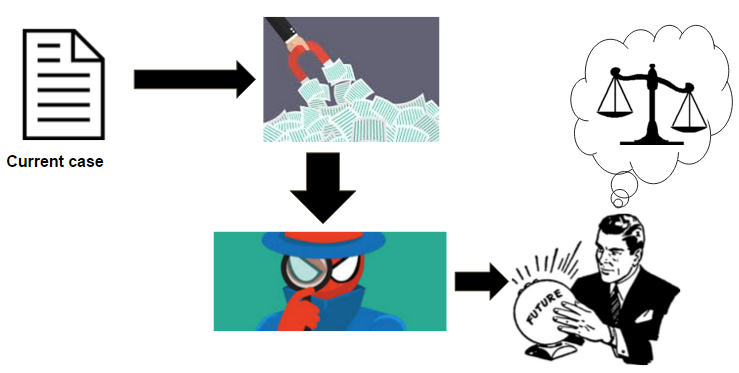
\includegraphics[width=0.7\textwidth]{lawyerwork.png}
\end{center}

\begin{block}{Pquoi?}
\begin{itemize}
\item comprendre et comparer l'application loi (contentieux, ville, ...)
\item estimer le risque judiciaire
\item ... %anticiper les affaires futures
\end{itemize}
\end{block}
\end{frame}

\begin{frame}{Motivation: documents non-structurés, langage complexe}
\scriptsize
\begin{columns}
\begin{column}{.50\linewidth}
ARRÊT N°

R.G: 11/03924

...

{C D'APPEL} DE {NÎMES}

{CHAMBRE CIVILE}

{1ère Chambre A}

ARRÊT DU {20 MARS 2012}

APPELANTE:

{Madame Michéle A.} ...

assistée de la {SELARL VAJOU}, ...

INTIMES:

{Monsieur Martial B} ...

assisté de la {SCP MARION GUIZARD PATRICIA SERVAIS}, ...

COMPOSITION DE LA C LORS DU DÉLIBÉRÉ:

{M. Dominique BRUZY, Président}

{M. Serge BERTHET, Conseiller}

...
\end{column}
\begin{column}{.50\linewidth}
FAITS, PROCEDURE, ...

Madame Michèle A. demande:

...

- de condamner Madame JONES-B. à lui payer la somme de {2.500 euros} au titre de l'{article 700 du Code de Procédure Civile}, 

\vspace{0.4cm}

PAR CES MOTIFS, LA C:

...

Vu l'{article 809 du Code de Procédure Civile},

...

{Déboute Madame A. de sa demande de provision sur dommages-intérêts.}

...

Vu l'{article 700 du Code de Procédure Civile},

Condamne Madame JONES-B. à verser à Madame A. la somme de {2.500 euros}.
\end{column}
\end{columns}
\end{frame}

\begin{frame}[c]{Motivation: grand volume de décisions}
\textbf{Plus de 4 millions de décisions prononcées / an}
\begin{table}[!htb]
{
\footnotesize
\begin{center}
\begin{tabular}{|p{2cm}|c|c|c|c|c|}
\hline
 & \textbf{2010} & \textbf{2011} & \textbf{2012} & \textbf{2013} & \textbf{2014} \\
 \hline
 \textbf{Justice civile} & 2 673 131  & 2 654 179 & 2 647 813 & 2 761 554  & 2 618 374 \\
 \hline
Justice pénale & 1 173 242 & 1 180 586 & 1 251 979 & 1 303 469 & 1 203 339 \\
 \hline
 Justice administrative & 224 787 & 225 608 & 228 680 & 221 882 & 230 477 \\
 \hline
\end{tabular}

\textit{\tiny{Sce: \url{http://www.justice.gouv.fr/budget-et-statistiques-10054/chiffres-cles-de-la-justice-10303/}}}  
\end{center}
}
\caption{Nombre de décisions prononcées en France par an}\label{decisionstats}
\end{table}
\end{frame}

\begin{frame}[t]{Motivation: recherches et analyses sémantiques difficiles}

Moteurs de recherche juridique à mots-clés 

Pas d'analyse synthétique des décisions 

%\begin{figure}
\fbox{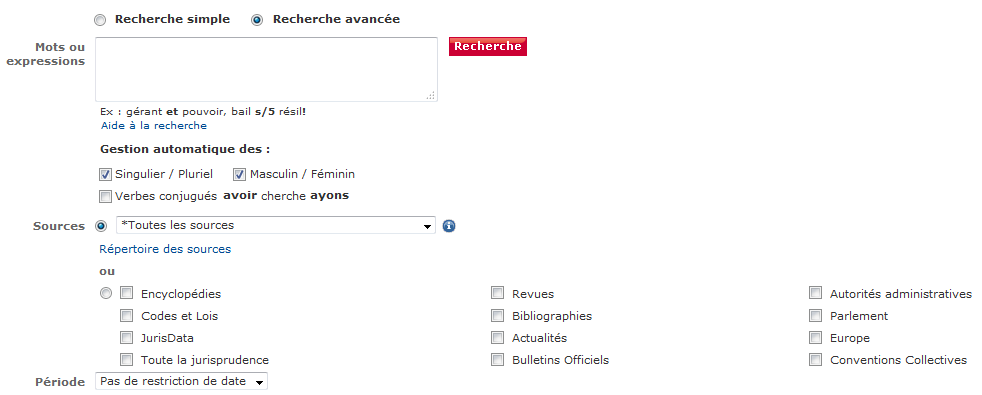
\includegraphics[width=0.9\paperwidth]{jurica.png}}

\textit{\tiny{Sce: \url{LexisNexis.com}}} 
%\caption{Formulaire de recherche}
%\end{figure}
\end{frame}

\begin{frame}{Objectif: Moteur d'analyse sémantique}
Stage été 2017 [ PRYSIAZHNIUK Anastasiia ]
\begin{center}
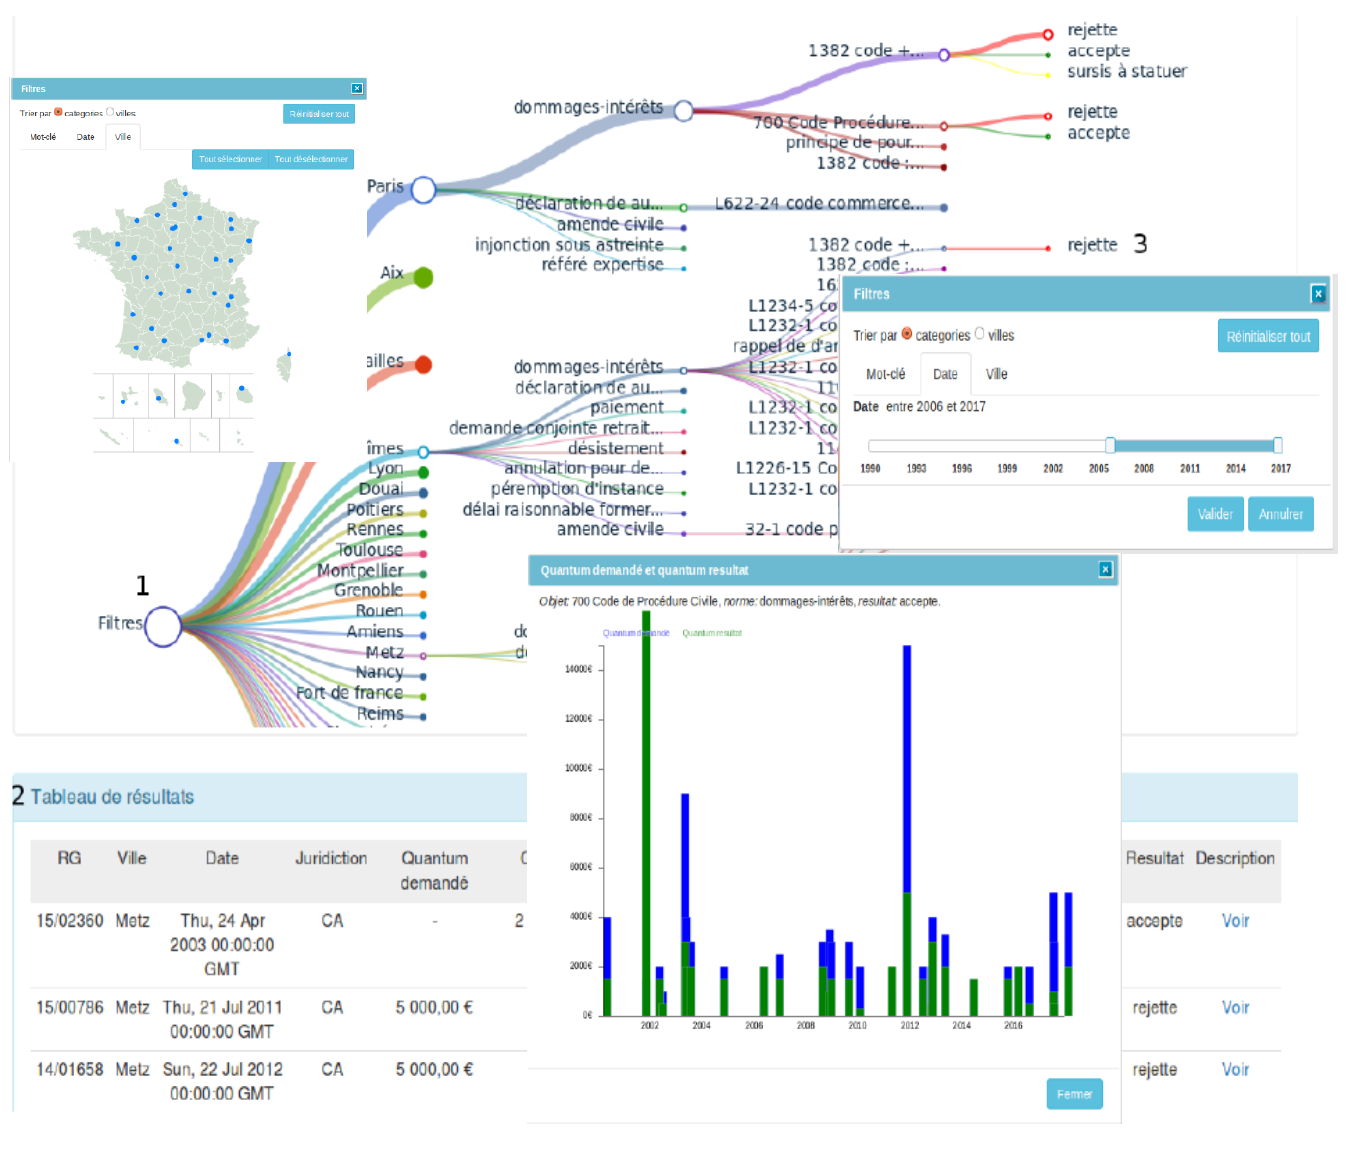
\includegraphics[width=0.75\textwidth]{interface.png}
\end{center}
\end{frame}

%\begin{frame}{Pipeline d'analyse sémantique}
%\centering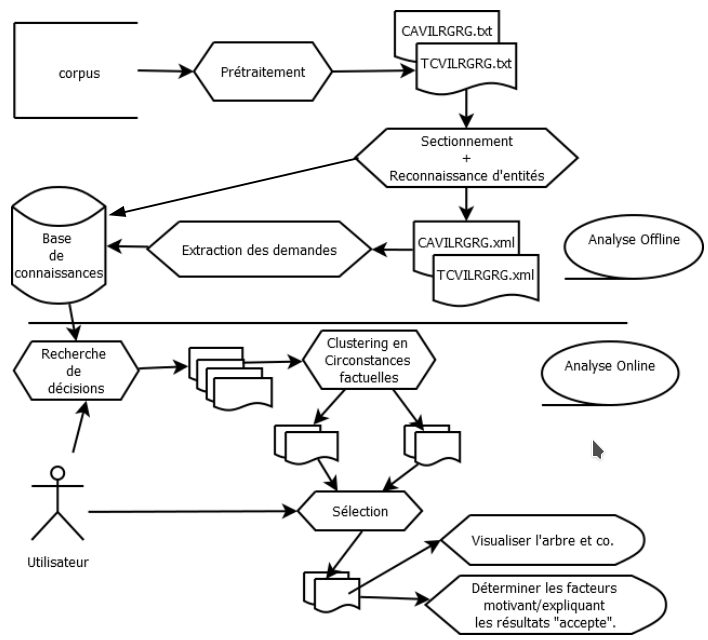
\includegraphics[width=0.75\textwidth]{pipelineComplet.png}
%\end{frame}

\begin{frame}{Problématiques d'extraction d'information}
\centering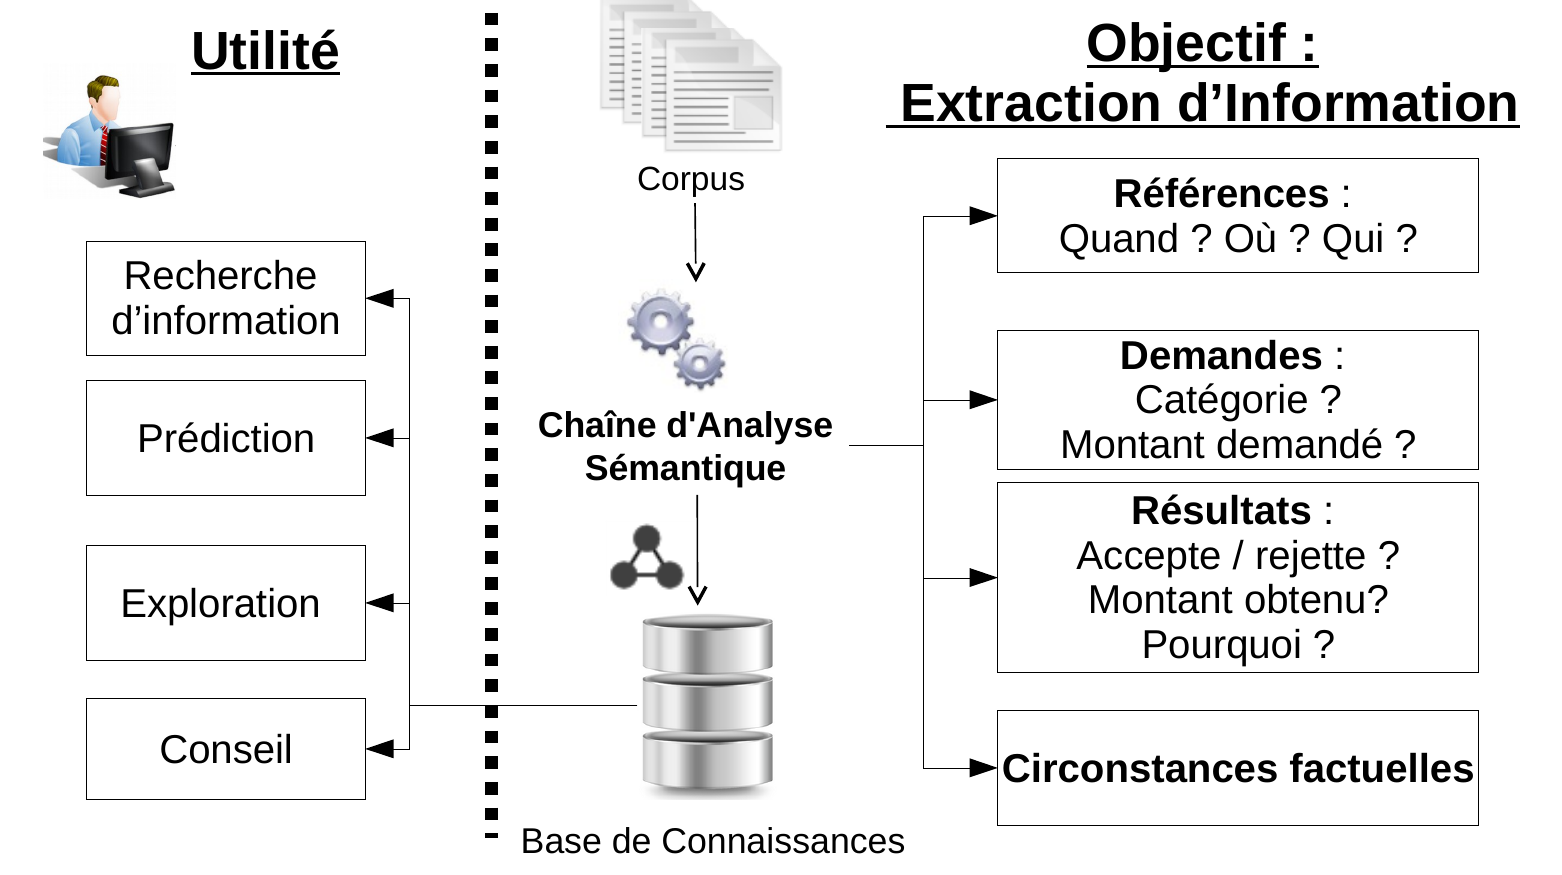
\includegraphics[width=\textwidth]{summary-prj.png}
\end{frame}


\section{Extraction des demandes par pondération de termes clef et zonage}
\subsection{Motivation}
\begin{frame}{T\^ache: extraire les quanta et le sens du résultat}
\scriptsize
Expressions non structurées, par  \textcolor{orange}{référence}, par \textcolor{blue}{agrégation}
\begin{exampleblock}{Expression de demande et resultat}
%danais/CASAI1401082.xml
\scriptsize
Jennifer M. , Catherine M. et Sandra M. ... demandent à la C de ' :

- \textcolor{orange}{infirmer le dit jugement en toutes ses dispositions} ; ...

Statuant à nouveau ...

- les condamner au paiement d' une somme de  \textbf{3 000,00 € pour procédure abusive} et
aux entiers dépens ; ...

La c, ...  
CONFIRME \textcolor{orange}{le jugement entreprise} en \textcolor{blue}{toutes ses dispositions}.

\end{exampleblock}


\begin{table} 
\centering 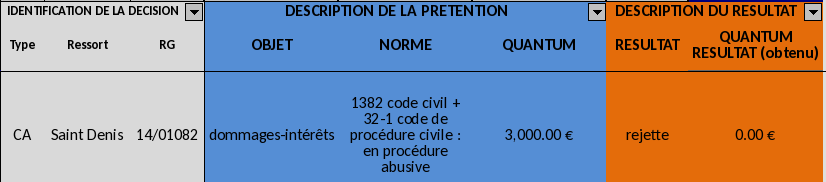
\includegraphics[width=0.9\textwidth]{tab-danais.png}
\caption{\scriptsize Informations à extraire (Dommages-intérêts pour procédure abusive)}
\end{table}
\end{frame}

\subsection{Formulation et décomposition du problème}

\begin{frame}{Décomposition du problème}
Problème décomposé en 3 tâches:
\begin{enumerate}
\item Identification des catégories présentes dans le document
\item Détection des quanta demandés, quantas obtenus, et sens du résultat
\item Liaison des informations relatives à la même demande
\end{enumerate}
\end{frame}

\subsection{Synthèse bibliographique}
% tâche semblable, méthodes récentes, pquoi ce n'est pas applicable à notre cas?
% Justification d'une méthode propre aux données qu'on a
\begin{frame}{Problèmes similaires: objectif des tâches}
%\scriptsize
\begin{itemize}
\item Extraction d'évènement : 
\end{itemize}
\begin{table}
\scriptsize
\begin{tabular}{|p{0.13\textwidth}|p{0.3\textwidth}|p{0.4\textwidth}|}
\hline
\textbf{Champs} & \textbf{\cite{ace2005event}} & \textbf{Analogie chez les demandes} \\ \hline
\textbf{Type} &  Die & Catégorie="Dommages-intérêts pour procédure abusive" \\ \hline
\textbf{Expression} (\textit{extend}) & "Il est \textbf{mort} hier d'une insuffisance rénale."  & (\textit{voir page précédente}) \\ \hline
\textbf{Déclencheur} & "mort" & "procédure abusive"\\ \hline
\textbf{Argument} & Victim-Arg="il" \linebreak Time-Arg="hier"  & Quantum-demandé="3000€"\linebreak  Quantum-obtenu="0 €"\ \\ \hline
\textbf{Attribut} & Polarity=POSITIVE, Tense=PAST & Sens-résultat="Rejeté" \\ \hline
\end{tabular}
\end{table}
\begin{itemize}
\item Remplissage de champs des entités \textbf{Demande} (\textit{slot-filling)}: \textbf{Catégorie, Quantum-demandé, Quantum-obtenu, Sens-résultat}
\item Extraction d'entités et relations: par ex. \textbf{(quantum demandé, quantum obtenu)}
\end{itemize}
\end{frame}

%\begin{frame}{Travaux similaires: Approches}
%\textbf{Méthodes à base de classifieurs}
%
%Par ex. une chaîne de classifieurs de mots (entropy maximal vs. plus-proches-voisins) \cite{ahn2006stages}
%\begin{enumerate}
%\item identification des déclencheurs: POS-tag, context avant et après, profondeur dans l'arbre de dépendance, ...
%\item identification des arguments:  déclencheur, type d'entité, chemin dans l'arbre de dépendance, ...
%\item affectation des attributs: \textit{la plupart des descripteurs de l'identification des déclencheurs}
%\end{enumerate}
%\end{frame}

\begin{frame}{Problèmes similaires: Approches}
\scriptsize
\begin{table}
\scriptsize
\begin{tabular}{|p{0.25\textwidth}|p{0.7\textwidth}|}
\hline
\textbf{Type d'approches} & \textbf{Exemples} \\ \hline
\textbf{Chaine de traitement} & \textbf{Chaîne de classifieurs  }\cite{ahn2006stages} \\ \hline
\textbf{Modélisation probabiliste} de la structure de l'évènement & \textbf{Modèle joint d'inférence} des entités, arguments, déclencheurs

$p_\theta(t_i, r_i, a \vert i, N_i, x)$ \cite{yang2016jointEntityEvt} %\linebreak 
\\ \hline
\textbf{Réseau de neuronnes} pour automatiser la génération des caractéristiques et la modélisation de la structure & (i) \textbf{Architecture multicouche de réseaux de neuronnes récurrents}: encodage de la phrase, encodage des contextes, prédiction du déclencheur, prédiction des rôles, mémoire matricielle d'interdépendance déclencheur-argument \cite{nguyen2016jointtrgarg},  

(ii) \textbf{Réseau de pointeur} (\textit{pointer network}): un encodeur de la phrase et des contextes, plusieurs décodeurs (un pour chaque champ) \cite{palm2017e2e-dnn} \\ \hline
\end{tabular}
\caption{\scriptsize Type d'approches}
\end{table}
\end{frame}

\begin{frame}{Difficultés liées à l'extraction des demandes}
\begin{alertblock}{}
\begin{itemize}
\item Présence de plusieurs demandes de catégories similaires et/ou différentes dans une m\^eme décision
\item Toutes les catégories ne sont pas connues d'avance (+500 catégories)
\item Difficile d'annoter une base d'évaluation pour toutes les couvrir
\end{itemize}
\end{alertblock}

\begin{block}{Il faut une approche :}
\begin{itemize}
\item qui s'adapte à la catégorie à extraire 
\item qui permette de rajouter de nouvelles catégories 
\end{itemize}
\end{block}
\end{frame}

\subsection{Description de l'approche proposée}
\begin{frame}{Architecture du pipeline d'extraction}
\begin{figure}
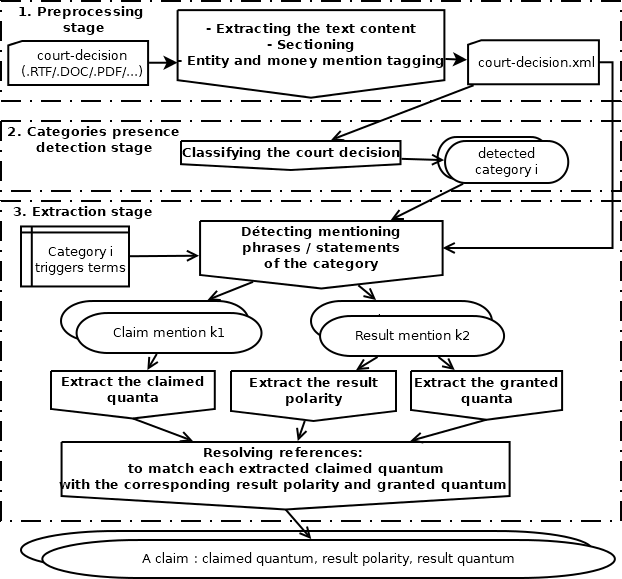
\includegraphics[width=0.7\textwidth]{pipeline-dmd.png}
\caption{Pipeline d'extraction d'analyse.}
\end{figure}
\end{frame}

\begin{frame}{Identification des passages et des informations}
Demande dans la section \textit{Litige} (Faits, procédures, et moyens des parties)

Résultat dans la section \textit{Dispositif}
\scriptsize
\begin{table}
 \begin{tabular}{|p{0.28\textwidth}|p{0.3\textwidth}|p{0.12\textwidth}|p{0.11\textwidth}|}
 \hline
 \textbf{Demande} & \multicolumn{3}{c|}{\textbf{Résultat} (organisé par polarité)} \\ \hline
  & \textbf{accepte}  &\textbf{sursis à statuer} & \textbf{rejette}  \\ \hline
 \textit{accorder, admettre, admission, allouer, condamnation, condamner, fixer, laisser, prononcer, ramener, surseoir} & \textit{accorde, accordons, admet, admettons, alloue, allouons, condamne, condamnons, déclare, déclarons, fixe, fixons, laisse, laissons, prononce, prononçons} & \textit{réserve, réservons, surseoit, sursoyons} & \textit{déboute, déboutons, rejette, rejettons} \\ \hline
 \end{tabular}
  \caption{Mots introduisant les énoncés de demandes et de résultats}\label{introducing-words}
 \end{table}
 
 
 \begin{figure}
 \begin{flushleft}
%" ... débouter M. S. de l' ensemble de ses demandes

- le \textbf{<demande categorie="acpa">}\underline{condamner} à payer une <trigger categorie="acpa">\textbf{amende civile}</trigger> de <argent> \textbf{1.500 euros} </argent> pour procédure abusive ...

- le\textbf{</demande>} \underline{condamner} à payer la somme ..."
\end{flushleft}
\caption{Exploiter la proximité entre triggers et sommes d'argent}\label{example-zone}
\end{figure} 
\end{frame}

\begin{frame}{Identification des passages et des informations(2)}
\begin{itemize}
\item Identification des passages: 
\begin{enumerate}
\item Soit par la seule \textbf{présence d'un trigger} : on zone aut des triggers 
\item Soit par \textbf{pondération des zones à argent}  : 
\begin{enumerate}
\item on zone aut des sommes d'argent
\item on pondère les zones (par ex. somme des poids des triggers)
\item on sélectionne une zone si elle a un poids $\geq$ \texttt{POIDS SEUIL}
\end{enumerate}
\end{enumerate}
\item Identification des informations:
\begin{enumerate}
\item quantum: somme d'argent près d'un trigger
\item sens du résultat : 
\begin{itemize}
\item soit en fonction du verbe introductif de l'énoncé du résultat
\item soit "\textit{rejette}" si pas d'énoncé du résultat
\end{itemize}
\end{enumerate}
\item Résolution des références:
\begin{itemize}
\item matching des énoncés (similarité textuelle)
\item matching des quanta (Hypothèse d'apparition dans le même ordre)
\end{itemize}
\end{itemize}
\end{frame}

\begin{frame}{Phase d'entrainement}
Catégorie  $c_i$, Corpus d'entrainement  $D = D_{c_i} \cup D_{\overline{c_i}} = \lbrace D_j\rbrace_{1\leq j\leq \vert D \vert}$
\begin{enumerate}
\item \textbf{Détecteur de catégorie: }
\begin{itemize}
\item vectoriser les décisions de la base d'entrainement: $w(t_k, D_j) = lw(t_k, D_j) \times gw(t_k) \times nf(D_j)$ \cite{salton1988term-weighting}
\item entrainer un algorithme de classification  (SVM, Naïf Bayésien, K plus proches voisins ...)
\end{itemize}
\item \textbf{Extracteur de triplets de quanta et sens du résultat:}
\begin{itemize}
\item Apprendre les triggers sur la base d'entrainement (passages à quanta vs. passages sans quanta)
\begin{enumerate}
\item pondération des termes $t_k$ avec une métrique de RI par ex. :

\text{Métrique non supervisée: } 

 $idf(t_k) = \log_2 (\frac{N}{N_{t_k}})$  \cite{sparck1972idf}

\text{Métriques supervisées : } 

 $gss(t_k,c_i) = (N_{t_k,c_i} N_{\overline{t_k},\overline{c_i}}) -  (N_{t_k,\overline{c_i}} N_{\overline{t_k},c_i})$ \cite{galavotti2000gss}

 $ngl(t_k,c_i) = \frac{\sqrt{N} ((N_{t_k,c_i} N_{\overline{t_k},\overline{c_i}}) - (N_{t_k,\overline{c_i}} N_{\overline{t_k},c_i}))}{\sqrt{N_{t_k} N_{\overline{t_k}} N_{c_i} N_{\overline{c_i}}}}$ \cite{ng1997ngl}
\item sélection des termes aux poids 
\end{enumerate}
\end{itemize}
\end{enumerate}
\end{frame}

\subsection{Résultats et discussions}

\begin{frame}{Données}
\begin{figure}
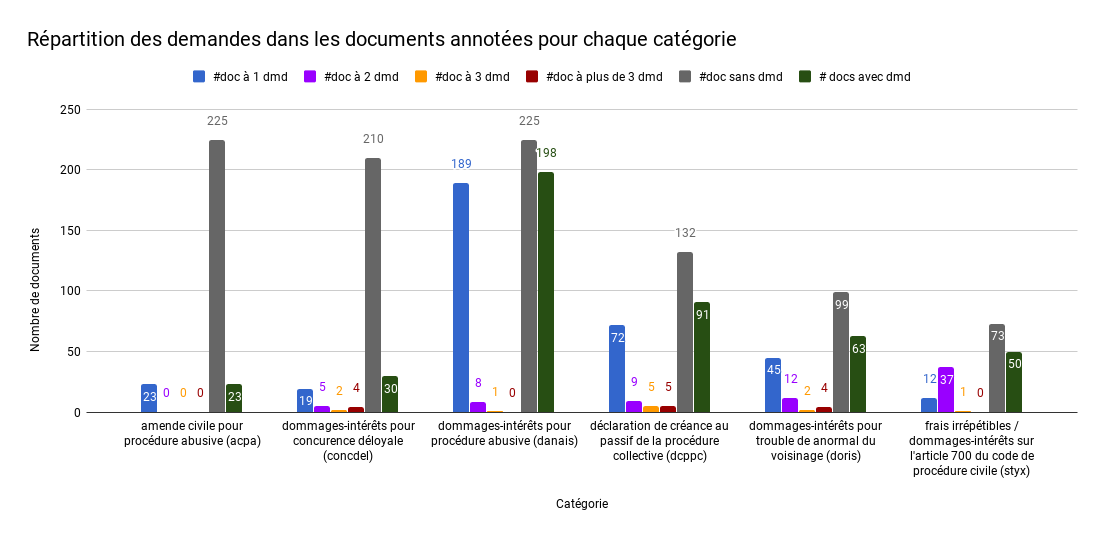
\includegraphics[width=\textwidth]{chartDataset.png}
%\caption{Répartitions des demandes dans les documents annotées pour chaque catégorie.}
\end{figure}
P chaque catégorie, plus de $50\%$ des documents annotées ont une seule demande. (\textbf{sauf pour l'article 700})
\end{frame}

\begin{frame}{Métriques d'évaluation}
Catégorie  $c_i$, tuple d'information $I \subseteq \lbrace Q_{DMD}, S_{RST}, Q_{RST} \rbrace $

Corpus d'évaluation  $D = D_{c_i} \cup D_{\overline{c_i}} = \lbrace D_j\rbrace_{1\leq j\leq \vert D \vert}$, où $D_j$  est un document

\scriptsize
\[\text{Nombre de vrais positifs (bons): } TP_{c_i,I,D} = \sum\limits^{\vert D \vert}_{j=1} TP_{c_i,I,D_j}\] 
\[\text{Nombre de faux positifs (en trop): } FP_{c_i,I,D} = \sum\limits^{\vert D \vert}_{j=1} FP_{c_i,I,D_j}\] 
\[\text{Nombre de faux négatifs (manqués): } FN_{c_i,I,D_j} = \sum\limits^{\vert D \vert}_{j=1} FN_{c_i,I,D_j}\]
\[Precision_{c_i,I,D} = \frac{TP_{c_i,I,D}}{TP_{c_i,I,D} + FP_{c_i,I,D}}\]
\[Rappel_{c_i,I,D} = \frac{TP_{c_i,I,D}}{TP_{c_i,I,D} + FN_{c_i,I,D}}\]

\[F1_{c_i,I,D} =2 \times \frac{Precision_{c_i,I,D} \times Rappel_{c_i,I,D}}{Precision_{c_i,I,D} + Rappel_{c_i,I,D}}\]


\end{frame}

\begin{frame}{Evaluation de la détection des catégories}
\begin{table}
\tiny
\caption{Resultats d'une 5-fold cross-validation sur $D$ pour la detection categorie  (P= Precision, R=Rappel, F1 = F1-mesure)}\label{best_classif_score}
\begin{tabular}{l|c@{\hskip 0.1in}lllc@{\hskip 0.1in}lllc@{\hskip 0.1in}lllc@{\hskip 0.1in}lll}
\hline\noalign{\smallskip}
       &   \multicolumn{3}{c}{Naïf Bayésien}    &    \multicolumn{3}{c}{Arbre de décision}   &  \multicolumn{3}{c}{KNN}  & \multicolumn{3}{c}{SVM}     \\       
\noalign{\smallskip}
\hline
\noalign{\smallskip}
  Category      & P     & R     & F1    & P     & R     & F1    & P     & R     & F1    & P     & R     & F1    \\        
\noalign{\smallskip}
\hline
\noalign{\smallskip}
acpa    & 1.0 & 1.0 & 1.0 & 0.996 & 0.955 & 0.972 & 1.0 & 1.0 & 1.0 & 0.996 & 0.955 & 0.972 \\
concdel & 1.0 & 1.0 & 1.0 & 1.0 & 1.0 & 1.0 & 1.0 & 1.0 & 1.0 & 0.995 & 0.967 & 0.979 \\
danais  & 0.988 & 0.989 & 0.988 & 0.996 & 0.995 & 0.995 & 0.995 & 0.995 & 0.995 & 0.993 & 0.993 & 0.993 \\
dcppc   & 1.0 & 1.0 & 1.0 & 1.0 & 1.0 & 1.0 & 1.0 & 1.0 & 1.0 & 1.0 & 1.0 & 1.0 \\
doris   & 1.0 & 1.0 & 1.0 & 1.0 & 1.0 & 1.0 & 1.0 & 1.0 & 1.0 & 1.0 & 1.0 & 1.0 \\
styx    & 1.0 & 1.0 & 1.0 & 0.984 & 0.983 & 0.983 & 1.0 & 1.0 & 1.0 & 1.0 & 1.0 & 1.0 \\
\hline
\end{tabular}
\end{table}
\end{frame}

\begin{frame}{Quelle métrique de pondération et quel zonage?}
\begin{table}[]
\tiny
\begin{flushleft}
\caption{Comparaison des métriques de pondération et des stratégies de zonage sur le corpus $D$ (F1-mesure sur l'extraction du tuple $(Q_{DMD},S_{RST}, Q_{RST})$)}
\label{my-label}
\begin{tabular}{l|ll|ll|ll|ll|ll|ll}
Métrique & \multicolumn{2}{c|}{acpa} &  \multicolumn{2}{c|}{concdel}  &  \multicolumn{2}{c|}{danais} &  \multicolumn{2}{c|}{dcppc} &  \multicolumn{2}{c|}{doris}   &  \multicolumn{2}{c}{styx}    \\ \noalign{\smallskip}
\hline
         & tp    & zw    & tp      & zw    & tp     & zw    & tp    & zw    & tp    & zw    & tp    & zw    \\ \noalign{\smallskip}
\hline
CHI2     & 0.683 & 0.698 & 0.061   & 0.061 & 0.443  & 0.411 & 0.259 & 0.264 & 0.187 & 0.071 & 0.321 & 0.366 \\
DBIDF    & 0.683 & 0.698 & 0.076   & 0.033 & 0.461  & 0.416 & 0.254 & 0.264 & 0.084 & 0     & 0.331 & 0.358 \\
DELTADF  & 0.683 & 0.698 & 0.144   & 0.082 & 0.443  & 0.41  & 0.259 & 0.264 & 0.143 & 0.142 & 0.334 & 0.281 \\
DSIDF    & 0.678 & 0.698 & 0.076   & 0.052 & 0.399  & 0.152 & 0.014 & 0     & 0.019 & 0     & 0.343 & 0.33  \\
GSS      & 0.683 & 0.698 & 0.144   & 0.082 & 0.443  & 0.41  & 0.259 & 0.264 & 0.143 & 0.142 & 0.334 & 0.281 \\
IDF      & 0.067 & 0     & 0.033   & 0     & 0.04   & 0     & 0     & 0     & 0     & 0     & 0     & 0     \\
IG       & 0.011 & 0.049 & 0.05    & 0.034 & 0.304  & 0.073 & 0     & 0     & 0.019 & 0     & 0.058 & 0     \\
KLD      & 0.432 & 0.398 & 0.146   & 0.124 & 0.459  & 0.409 & 0.252 & 0.254 & 0.158 & 0.154 & 0.243 & 0.42  \\
MAR      & 0.683 & 0.698 & 0.144   & 0.091 & 0.443  & 0.42  & 0.259 & 0.264 & 0.156 & 0.146 & 0.334 & 0.281 \\
NGL      & 0.683 & 0.698 & 0.061   & 0.034 & 0.443  & 0.411 & 0.259 & 0.264 & 0.122 & 0.02  & 0.321 & 0.347 \\
RF       & 0.683 & 0.698 & 0.202   & 0.043 & 0.491  & 0.367 & 0.242 & 0.21  & 0.101 & 0.058 & 0.387 & 0.351 \\ \hline
 \noalign{\smallskip}
\hline
Max        & 0.683 & \textbf{0.698} & \textbf{0.202}   & 0.124  & \textbf{0.491}  & 0.42  & 0.259 & \textbf{0.264} & \textbf{0.187} & 0.154 & 0.387 & \textbf{0.42} 
\end{tabular}

tp = zonage par la seule présence d'un trigger

zw = zonage par pondération des passages à somme d'argent
\end{flushleft}

\end{table}

La métrique et la stratégie de zonage dépendent de la catégorie

\end{frame}

\begin{frame}{Exemple de termes sélectionnés}
\scriptsize
\begin{table}
\begin{tabular}{ll|lp{0.28\textwidth}}
 \multicolumn{2}{c|}{concdel} &  \multicolumn{2}{c}{danais} \\ \hline \noalign{\smallskip}
 NGL & DSIDF & NGL & DSIDF \\ \hline
déloyale & concurrence déloyale & procédure abusive       & procédure abusive et injustifiée                  \\ \hline
perte    & déloyale             & 32-1                    & fondement de l ' article 32-1                     \\ \hline
actes    &                      & abusive                 & dommages-intérêts pour procédure abusive          \\ \hline
50.000   & agissements          & intérêts pour procédure & titre de dommages-intérêts pour procédure abusive
\end{tabular}
\end{table}

$ngl(t_k,c_i) = \frac{\sqrt{N} ((N_{t_k,c_i} N_{\overline{t_k},\overline{c_i}}) - (N_{t_k,\overline{c_i}} N_{\overline{t_k},c_i}))}{\sqrt{N_{t_k} N_{\overline{t_k}} N_{c_i} N_{\overline{c_i}}}}$

$dsidf(t_k, c_i)=\log (\frac{(N_{\overline{c_i}}N_{t_k,c_i}) + 0.5}{(N_{c_i}N_{t_k,\overline{c_i}}) + 0.5} $
\end{frame}

\begin{frame}{Entrainement avec sélection de la meilleure métrique (1)}
\begin{table}[!htbp]
\tiny
\begin{tabular}{|c|c|c|c|c|c|c|}
\hline
$c_i$ & Tuple d'info ($I$) &  $P_{c_i,I,D_{c_i}}$ & $R_{c_i,I,D_{c_i}}$ & $F1_{c_i,I,D_{c_i}}$ & Docs. Parfaits & \#extraits/\#attendus/$\vert D_{c_i}  \vert$\\ \hline
\multirow{4}{*}{acpa} & $(Q_{DMD})$ & 0.709 & 0.73 & 0.705 & \textcolor{red}{0.47} & \multirow{5}{*}{5.2/4.6/4.6} \\ 
 & $(S_{RST})$ & 0.691 & 0.7 & 0.683 & \textcolor{red}{0.48} &  \\ 
 & $(Q_{RST})$ & 0.72 & 0.74 & 0.716 & \textcolor{red}{0.48} &  \\ 
 & $(Q_{DMD},S_{RST}, Q_{RST})$ & 0.651 & 0.65 & 0.638 & \textcolor{red}{0.43} &  \\  \hline
\multirow{4}{*}{concdel}  & $(Q_{DMD})$ & \textcolor{red}{0.461} & \textcolor{red}{0.393} & \textcolor{red}{0.376} & \textcolor{red}{0.233} & \multirow{5}{*}{11.6/11.6/6.0} \\ 
 & $(S_{RST})$ & 0.544 & \textcolor{red}{0.442} & \textcolor{red}{0.427} & \textcolor{red}{0.2} &  \\ 
 & $(Q_{RST})$ & 0.595 & \textcolor{red}{0.482} & \textcolor{red}{0.465} & \textcolor{red}{0.2} &  \\ 
 & $(Q_{DMD},S_{RST}, Q_{RST})$ & \textcolor{red}{0.337} & \textcolor{red}{0.299} & \textcolor{red}{0.28} & \textcolor{red}{0.167} &  \\  \hline
 \multirow{4}{*}{danais} & $(Q_{DMD})$ & 0.548 & 0.516 & 0.527 & \textcolor{red}{0.346} & \multirow{4}{*}{36.6/38.8/37.0} \\ 
 & $(S_{RST})$ & 0.69 & 0.646 & 0.661 & \textcolor{red}{0.454} &  \\ 
 & $(Q_{RST})$ & 0.714 & 0.666 & 0.682 & \textcolor{red}{0.465} &  \\ 
 & $(Q_{DMD},S_{RST}, Q_{RST})$ & \textcolor{red}{0.482} & \textcolor{red}{0.46} & \textcolor{red}{0.466} & \textcolor{red}{0.314} &  \\  \hline
\multirow{4}{*}{dcppc} & $(Q_{DMD})$ & \textcolor{red}{0.334} & \textcolor{red}{0.392} & \textcolor{red}{0.358} & \textcolor{red}{0.217} & \multirow{4}{*}{26.8/22.2/16.6} \\ 
 & $(S_{RST})$ & 0.665 & 0.798 & 0.721 & 0.544 &  \\ 
 & $(Q_{RST})$ & 0.62 & 0.744 & 0.672 & 0.509 &  \\ 
 & $(Q_{DMD},S_{RST}, Q_{RST})$ & \textcolor{red}{0.22} & \textcolor{red}{0.26} & \textcolor{red}{0.237} & \textcolor{red}{0.181} &  \\  \hline
 \multirow{4}{*}{doris} & $(Q_{DMD})$ & \textcolor{red}{0.279} & \textcolor{red}{0.373} & \textcolor{red}{0.314} & \textcolor{red}{0.033} & \multirow{4}{*}{26.8/20.0/12.4} \\ 
 & $(S_{RST})$ & \textcolor{red}{0.391} & 0.524 & \textcolor{red}{0.439} & \textcolor{red}{0.146} &  \\ 
 & $(Q_{RST})$ & \textcolor{red}{0.329} & \textcolor{red}{0.414} & \textcolor{red}{0.361} & \textcolor{red}{0.131} &  \\ 
 & $(Q_{DMD},S_{RST}, Q_{RST})$ & \textcolor{red}{0.177} & \textcolor{red}{0.229} & \textcolor{red}{0.197} & \textcolor{red}{0.017} &  \\  \hline
\multirow{4}{*}{styx} & $(Q_{DMD})$ & 0.762 & 0.642 & 0.695 & \textcolor{red}{0.46} & \multirow{4}{*}{15.0/17.8/10.0} \\ 
 & $(S_{RST})$ & 0.701 & 0.593 & 0.64 & \textcolor{red}{0.34} &  \\ 
 & $(Q_{RST})$ & 0.824 & 0.696 & 0.752 & \textcolor{red}{0.46} &  \\ 
 & $(Q_{DMD}, Q_{RST}, S_{RST})$ & \textcolor{red}{0.44} & \textcolor{red}{0.372} & \textcolor{red}{0.402} & \textcolor{red}{0.28} &  \\  \hline
\end{tabular} 
%{
%\tiny
%$I = \lbrace \text{$Q_{DMD}$, $S_{RST}$, $Q_{RST}$} \rbrace$; DMD = "demande", RST = "résultat"
%
%$\text{$(Q_{DMD},S_{RST}, Q_{RST})$} = I$; $\text{RST COMPLET} = \lbrace \text{$S_{RST}$, $Q_{RST}$} \rbrace$
%
%\#dp et \#dg = nombre de demandes resp. prédites et de la vérité terrain; $\vert D \vert$: nombre de documents du dataset
%
%\textit{Train} = dataset d'apprentissage des déclencheurs; \textit{Test} = dataset de test; 
%P, R, F1 = resp. $Precision_{I_s}, Rappel_{I_s}, F1_{I_s}$ ;
%
%Doc = proportion de Documents pour lesquels toutes les infos de type $I_s$ ont été complètement bien identifiées
%
%Code couleur: \textcolor{blue}{bleu} = mesure >= 0.85,  \textcolor{red}{rouge} = mesure < 0.5
%}
%\end{center}
%P, R, F1 = resp. $Precision_{c_i,I,D}, Rappel_{c_i,I,D}, F1_{c_i,I,D}$
\caption{\scriptsize Zonage par la seule présence d'un trigger (sur le corpus $D_{c_i}$)}\label{resultats-mult-dmd-doc-level}
\end{table}
\end{frame}


\begin{frame}{Entrainement avec sélection de la meilleure métrique (2)}
\begin{table}[!htbp]
%\begin{center}
%\scriptsize 
\tiny
\begin{tabular}{|c|c|c|c|c|c|c|}
\hline
$c_i$ & Tuple d'info ($I$) &  $P_{c_i,I,D_{c_i}}$ & $R_{c_i,I,D_{c_i}}$ & $F1_{c_i,I,D_{c_i}}$ & Docs. Parfaits & \#extraits/\#attendus/$\vert D_{c_i}  \vert$\\ \hline
\multirow{4}{*}{acpa}  & $(Q_{DMD})$ & 0.753 & 0.61 & 0.672 & 0.57 & \multirow{5}{*}{3.8/4.6/4.6} \\ 
 & $(S_{RST})$ & \textcolor{blue}{0.92} & 0.74 & 0.818 & 0.7 &  \\ 
 & $(Q_{RST})$ & \textcolor{blue}{0.92} & 0.74 & 0.818 & 0.7 &  \\ 
 & $(Q_{DMD},S_{RST}, Q_{RST})$ & 0.753 & 0.61 & 0.672 & 0.57 &  \\  \hline
\multirow{4}{*}{concdel}  & $(Q_{DMD})$ & \textcolor{red}{0.343} & \textcolor{red}{0.128} & \textcolor{red}{0.11} & \textcolor{red}{0.067} & \multirow{5}{*}{5.6/11.6/6.0} \\ 
 & $(S_{RST})$ & 0.535 & \textcolor{red}{0.15} & \textcolor{red}{0.17} & \textcolor{red}{0.067} &  \\ 
 & $(Q_{RST})$ & 0.543 & \textcolor{red}{0.17} & \textcolor{red}{0.182} & \textcolor{red}{0.067} &  \\ 
 & $(Q_{DMD},S_{RST}, Q_{RST})$ & \textcolor{red}{0.135} & \textcolor{red}{0.098} & \textcolor{red}{0.079} & \textcolor{red}{0.033} &  \\   \hline
 \multirow{4}{*}{danais} & $(Q_{DMD})$ & 0.66 & \textcolor{red}{0.296} & \textcolor{red}{0.395} & \textcolor{red}{0.227} & \multirow{5}{*}{17.8/38.8/37.0} \\ 
 & $(S_{RST})$ & 0.732 & \textcolor{red}{0.328} & \textcolor{red}{0.438} & \textcolor{red}{0.27} &  \\ 
 & $(Q_{RST})$ & 0.77 & \textcolor{red}{0.348} & \textcolor{red}{0.464} & \textcolor{red}{0.276} &  \\ 
 & $(Q_{DMD},S_{RST}, Q_{RST})$ & 0.61 & \textcolor{red}{0.276} & \textcolor{red}{0.367} & \textcolor{red}{0.216} &  \\  \hline
\multirow{4}{*}{dcppc} & $(Q_{DMD})$ & \textcolor{red}{0.391} & \textcolor{red}{0.363} & \textcolor{red}{0.372} & \textcolor{red}{0.252} & \multirow{5}{*}{21.4/22.2/16.6} \\ 
 & $(S_{RST})$ & 0.732 & 0.688 & 0.703 & 0.532 &  \\ 
 & $(Q_{RST})$ & 0.665 & 0.624 & 0.638 & \textcolor{red}{0.471} &  \\ 
 & $(Q_{DMD},S_{RST}, Q_{RST})$ & \textcolor{red}{0.275} & \textcolor{red}{0.248} & \textcolor{red}{0.259} & \textcolor{red}{0.204} &  \\  \hline
 \multirow{4}{*}{doris} & $(Q_{DMD})$ & \textcolor{red}{0.211} & \textcolor{red}{0.146} & \textcolor{red}{0.171} & \textcolor{red}{0.064} & \multirow{5}{*}{9.8/20.0/12.4} \\ 
 & $(S_{RST})$ & \textcolor{red}{0.418} & \textcolor{red}{0.217} & \textcolor{red}{0.268} & \textcolor{red}{0.114} &  \\ 
 & $(Q_{RST})$ & \textcolor{red}{0.342} & \textcolor{red}{0.166} & \textcolor{red}{0.211} & \textcolor{red}{0.096} &  \\ 
 & $(Q_{DMD},S_{RST}, Q_{RST})$ & \textcolor{red}{0.095} & \textcolor{red}{0.067} & \textcolor{red}{0.078} & \textcolor{red}{0.017} &  \\ \hline
\multirow{4}{*}{styx} & $(Q_{DMD})$ & 0.838 & 0.632 & 0.718 & 0.52 & \multirow{5}{*}{13.2/17.8/10.0} \\ 
 & $(S_{RST})$ & 0.772 & 0.571 & 0.654 & \textcolor{red}{0.36} &  \\ 
 & $(Q_{RST})$ & 0.786 & 0.583 & 0.666 & \textcolor{red}{0.38} &  \\ 
 & $(Q_{DMD},S_{RST}, Q_{RST})$ & 0.573 & \textcolor{red}{0.44} & \textcolor{red}{0.496} & \textcolor{red}{0.32} &  \\ \hline
\end{tabular} 
%{
%\tiny
%$I = \lbrace \text{$Q_{DMD}$, $S_{RST}$, $Q_{RST}$} \rbrace$; DMD = "demande", RST = "résultat"
%
%$\text{$(Q_{DMD},S_{RST}, Q_{RST})$} = I$; $\text{RST COMPLET} = \lbrace \text{$S_{RST}$, $Q_{RST}$} \rbrace$
%
%\#dp et \#dg = nombre de demandes resp. prédites et de la vérité terrain; $\vert D \vert$: nombre de documents du dataset
%
%\textit{Train} = dataset d'apprentissage des déclencheurs; \textit{Test} = dataset de test; 
%P, R, F1 = resp. $Precision_{I_s}, Rappel_{I_s}, F1_{I_s}$ ;
%
%Doc = proportion de Documents pour lesquels toutes les infos de type $I_s$ ont été complètement bien identifiées
%
%Code couleur: \textcolor{blue}{bleu} = mesure >= 0.85,  \textcolor{red}{rouge} = mesure < 0.5
%}
%\end{center}
%P, R, F1 = resp. $Precision_{c_i,I,D}, Rappel_{c_i,I,D}, F1_{c_i,I,D}$
\caption{\scriptsize Zonage par pondération des passages à somme d'argent (sur le corpus $D_{c_i}$)
}\label{resultats-mult-dmd-doc-level}
\end{table}
\end{frame}

%-=-=-=-=-=-=-=-=-=-=-=-=-=-=-=-=-=-=-=-=-=-=-=-=
%	Section: 
%-=-=-=-=-=-=-=-=-=-=-=-=-=-=-=-=-=-=-=-=-=-=-=-=

\section{Classification binaire pour identifier le sens du résultat}

\subsection{Restriction et motivations}
\begin{frame}{Restriction et motivation}
\begin{itemize}
\item Uniquement les décisions à une demande de la catégorie considérée
\begin{itemize}
\item Raison: plus de $50\%$ des documents dans la majorité des catégories
\end{itemize}
\item Classification binaire
\begin{itemize}
\item Raison: le sens d'un résultat est pratiquement toujs une de ces deux valeurs : \textbf{accepte} ou \textbf{rejette}
\end{itemize}
\end{itemize}
\begin{figure}
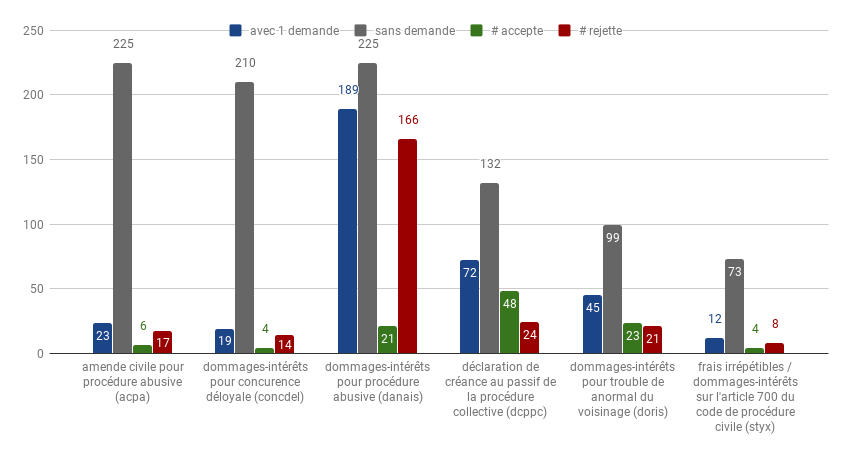
\includegraphics[width=0.8\textwidth]{chartDataset1dmd.png}
%\caption{\scriptsize Répartitions des sens de résultats (cas à une demande de la catégorie).}
\end{figure}
\end{frame}

%\subsection{Formulation et décomposition du problème}
%\begin{frame}{}
%
%\end{frame}
\subsection{Synthèse bibliographique}
% t^ache semblable, méthodes récentes, pquoi ce n'est pas applicable à notre cas?
% Justification d'une méthode propre aux données qu'on a

\begin{frame}{NBSVM \cite{wang2012nbsvm}}
$x^{(k)} = f^{(k)}$ vecteur intitial des caractéristiques du texte $k$

$r = \log \left( \frac{p/\vert\vert p \vert\vert_1}{q / \vert\vert q \vert\vert_1}\right)$, vecteur poids du classifieur bayésien multinomial

avec $p=\alpha + \sum_{i:y^{(i)}=1f^{(i)}}$, $q=\alpha + \sum_{i:y^{(i)}=-1f^{(i)}}$

L'idée: transformer les caractéristiques réduites à leur simple présence $\widehat{f}^{(k)}$ avec $r$ ($\overset{\sim}{f}^{(k)} = \widehat{r} \circ \widehat{f}^{(k)}$)

$\widehat{r}$ est calculé avec $\widehat{f}^{(k)}$

les nouveaux $x^{(k)} = \overset{\sim}{f}^{(k)}$ sont utilisés dans un SVM.

\end{frame}

\begin{frame}{fastText \cite{grave2017fastText}}
\begin{figure}
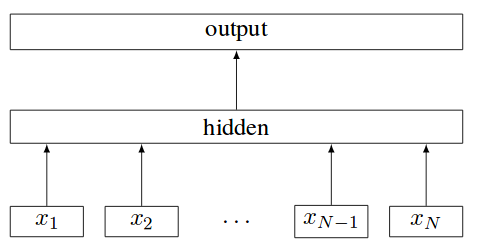
\includegraphics[width=0.5\textwidth]{fastTextArchi.png}
\caption{\scriptsize Architecture similaire au model CBOW : le label remplace le mot au milieu.}
\end{figure}

Entrainement : $min \left(-\frac{1}{N}y_n \cdot \sum\limits_{n=1}^N y_n \cdot \log{f(B\cdot A\cdot x_n)}\right)$ 

où $f$ est la fonction softmax $f(z) = \left[ \frac{e^{z_j}}{\sum\limits_{k=1}^K e^{z_k}} \right]_{\forall j \in \lbrace 1, ..., K \rbrace} $
\end{frame}

\begin{frame}{Résultats obtenus avec fastText et NBSVM}
\textbf{Influence du déséquilibre et de la (très) faible taille des données}
\begin{table}
\scriptsize
\begin{tabular}{|l|l|l|l|l|l|l|l|l|}
\hline
\textbf{Cat. Dmd.} & \textbf{Algo.} & \textbf{Préc.}   & \textbf{Préc. équi.} & \textbf{err-0} & \textbf{err-1} & \textbf{f1-0}  & \textbf{f1-1}  & \textbf{f1-macro-avg} \\ \hline
\textbf{dcppc}       & nbsvm      & 0.875 & 0.812        & 0.375 & 0     & 0.752 & 0.916 & \textbf{0.834}        \\ \hline
danais      & fasttext   & \textbf{0.888} & 0.5          & 1     & 0     & 0     & 0.941 & 0.47         \\ \hline
danais      & nbsvm      & 0.888 & 0.5          & 0     & 1     & 0.941 & 0     & 0.47         \\ \hline
concdel     & fasttext   & 0.775 & 0.5          & 1     & 0     & 0     & 0.873 & 0.437        \\ \hline
concdel     & nbsvm      & 0.775 & 0.5          & 0     & 1     & 0.873 & 0     & 0.437        \\ \hline
acpa        & fasttext   & 0.745 & 0.5          & 1     & 0     & 0     & 0.853 & 0.426        \\ \hline
acpa        & nbsvm      & 0.745 & 0.5          & 0     & 1     & 0.853 & 0     & 0.426        \\ \hline
doris       & nbsvm      & 0.5   & 0.492        & 0.85  & 0.167 & 0.174 & 0.63  & 0.402        \\ \hline
dcppc       & fasttext   & 0.667 & 0.5          & 0     & 1     & 0.8   & 0     & 0.4          \\ \hline
styx        & fasttext   & 0.667 & 0.5          & 1     & 0     & 0     & 0.8   & 0.4          \\ \hline
styx        & nbsvm      & 0.667 & 0.5          & 0     & 1     & 0.8   & 0     & 0.4          \\ \hline
doris       & fasttext   & 0.523 & 0.5          & 0     & 1     & 0.686 & 0     & 0.343        \\ \hline
\end{tabular}

\end{table}
0 == accepte

1 == rejette

\end{frame}

%\begin{frame}{Extension de la Régression PLS: Gini-PLS}
%Combinaison du Gini et du PLS1 (unilabel) \cite{souissi2013gini}:
%\begin{enumerate}
%\setlength\itemsep{1.5em}
%\item PLS (Régression partielle des moindres carrés): réduction supervisée des dimensions $x_1, x_2, ..., x_p$ en composantes orthogonales $t_1, ...., t_h$
%
%$t_h = w_{h1} x_1 + \cdots + w_{hj} x_j + \cdots + w_{hp} x_p$
%
%avec $w_{hj} = \frac{cov(u_{(h-1)j}, \epsilon_h)}{\sqrt{\sum_p^{j=1} cov^2(u_{(h-1)j}, \epsilon_h)}}$
%, $y=c_1 t_1 + ... + c_h t_h + \epsilon_h$,
%
%et $x_j=\beta_{1j} t_1 + ... + \beta_{hj} t_h + u_{(h-1)j}$
%
%\item Gini: élimination de la sensibilité au \textit{outliers} en remplaçant la covariance $cov(x_j, y)$ par la covariance de Gini $cog(y; x_j) := cov(y; R(x_j))$
%\end{enumerate}
%
%\end{frame}

\begin{frame}{Application des extensions de la Régression PLS (1)}
 PLS standard (Régression partielle des moindres carrés) 
 
 Réduction supervisée des dimensions $x_1, x_2, ..., x_p$ en composantes orthogonales $t_1, ...., t_h$

$t_h = w_{h1} x_1 + \cdots + w_{hj} x_j + \cdots + w_{hp} x_p$

avec $w_{hj} = \frac{cov(u_{(h-1)j}, \epsilon_h)}{\sqrt{\sum_p^{j=1} cov^2(u_{(h-1)j}, \epsilon_h)}}$
, $y=c_1 t_1 + ... + c_h t_h + \epsilon_h$,

et $x_j=\beta_{1j} t_1 + ... + \beta_{hj} t_h + u_{(h-1)j}$


\end{frame}

\begin{frame}{Application des extensions de la Régression PLS (2)}

\begin{enumerate}
\setlength\itemsep{1.5em}

\item Gini-PLS: 
élimination de la sensibilité au \textit{outliers} en remplaçant la covariance $cov(x_j, y)$ par la covariance de Gini $cog(y; x_j) := cov(y; R(x_j))$ pour l'estimation des résidus $u_{(h)j}$ et des poids $w_{hj}$ \cite{souissi2013gini}

\item Logit-PLS:  $\forall j > 1$, les $w_{hj} $ sont les coefficients de la régression logistique de $y$ sur les composantes $t_1, ..., t_{h-1}, u_{(h-1)j}$ \cite{tenenhaus2005logitpls}

\item Gini-Logit-PLS: covariance Gini pour $u_{(h)j}$ et coefficient Logit pour les $w_{hj}$
\end{enumerate}
\end{frame}


\begin{frame}{Résultats: meilleures configurations}
\begin{table}[]
\tiny
\label{my-label}
\begin{tabular}{|l|l|l|l|l|l|l|l|l|l|}
\hline
\textbf{Vecteur} & \textbf{classifieur} & \textbf{F1} & \textbf{min} & \textbf{Cat. min} & \textbf{max} & \textbf{Cat. max} & \textbf{F1 - 1$^{er}$F1} & \textbf{max - min} & \textbf{rang} \\ \hline
GSS*TF                 & Tree                & \textbf{0.668}     & 0.5                 & doris                  & 0.92               & dcppc                 & \textbf{0}                    & \textbf{0.42}           & 1             \\ \hline
AVG-G*TF      & LogitPLS         & \textbf{0.648}     & 0.518               & danais                 & 0.781              & dcppc                 & \textbf{0.02}                 & \textbf{0.263}          & 13            \\ \hline
AVG-G*TF      & StandardPLS      & \textbf{0.636}     & 0.49                & danais                 & 0.836              & dcppc                 & \textbf{0.032}                & \textbf{0.346}          & 24            \\ \hline
DELTADF*TF             & GiniPLS          & \textbf{0.586}     & 0.411               & danais                 & 0.837              & dcppc                 & \textbf{0.082}                & \textbf{0.426}          & 169           \\ \hline
DELTADF*TF             & GiniLogitPLS     & \textbf{0.578}     & 0.225               & styx                   & 0.772              & dcppc                 & \textbf{0.09}                 & \textbf{0.547}          & 220           \\ \hline
\end{tabular}
AVG-G == Moyenne des métriques globales de pondération
\end{table}
\scriptsize

En moyenne, la meilleure zone est la partie principale (litige\_motifs\_dispositif)

Les extensions du PLS ne sont pas très éloignées (si on choisi le bon shéma de vectorisation)

\end{frame}

\begin{frame}{Résultats pour chaque classe}
\begin{table}[]
\tiny
\centering
\label{my-label}
\begin{tabular}{|l|l|l|l|l|}
\hline
\textbf{Cat. Dmd} & \textbf{zone}                                    & \textbf{Vecteur}      & \textbf{classifieur} & \textbf{F1}    \\ \hline
\textbf{acpa}     & \textbf{demande\_resultat\_a\_resultat\_context} & \textbf{DBIDF*TF}           & \textbf{Tree}        & \textbf{0.846} \\ \hline
acpa              & litige\_motifs\_dispositif                       & DELTADF*TF                  & StandardPLS       & 0.697          \\ \hline
acpa              & litige\_motifs\_dispositif                       & AVERAGEGlobals*TF           & LogitPLS          & 0.683          \\ \hline
\textbf{concdel}  & \textbf{litige\_motifs\_dispositif}              & \textbf{GSS*TF}             & \textbf{Tree}        & \textbf{0.798} \\ \hline
concdel           & motifs                                           & IDF*TF                      & GiniLogitPLS      & 0.703          \\ \hline
concdel           & context                                          & DBIDF*LOGAVE                & StandardPLS       & 0.657          \\ \hline
\textbf{danais}   & \textbf{demande\_resultat\_a\_resultat\_context} & \textbf{CHI2*AVERAGELocals} & \textbf{Tree}        & \textbf{0.813} \\ \hline
danais            & demande\_resultat\_a\_resultat\_context          & AVERAGEGlobals*ATF          & LogitPLS          & 0.721          \\ \hline
danais            & demande\_resultat\_a\_resultat\_context          & AVERAGEGlobals*ATF          & StandardPLS       & 0.695          \\ \hline
\textbf{dcppc}    & \textbf{demande\_resultat\_a\_resultat\_context} & \textbf{CHI2*TF}            & \textbf{Tree}        & \textbf{0.985} \\ \hline
dcppc             & demande\_resultat\_a\_resultat\_context          & CHI2*TF                     & LogitPLS          & 0.94           \\ \hline
dcppc             & litige\_motifs\_dispositif                       & MARASCUILO*TP               & StandardPLS       & 0.934          \\ \hline
\textbf{doris}    & \textbf{litige\_motifs\_dispositif}              & \textbf{DSIDF*TP}           & \textbf{GiniPLS}  & \textbf{0.806} \\ \hline
doris             & litige\_motifs\_dispositif                       & DSIDF*TP                    & GiniLogitPLS      & 0.806          \\ \hline
doris             & litige\_motifs\_dispositif                       & IG*ATF                      & StandardPLS       & 0.772          \\ \hline
\textbf{styx}     & \textbf{motifs}                                  & \textbf{DSIDF*TF}           & \textbf{Tree}        & \textbf{1}     \\ \hline
styx              & demande\_resultat\_a\_resultat\_context          & DSIDF*LOGAVE                & GiniLogitPLS      & 0.917          \\ \hline
styx              & litige\_motifs\_dispositif                       & RF*TF                       & GiniPLS           & 0.833          \\ \hline
\end{tabular}
\end{table}

De bonnes performances si on varie les métaparamètres en fonction de la catégorie de demande
\end{frame}

%-=-=-=-=-=-=-=-=-=-=-=-=-=-=-=-=-=-=-=-=-=-=-=-=
%	Conclusion: 
%-=-=-=-=-=-=-=-=-=-=-=-=-=-=-=-=-=-=-=-=-=-=-=-=

\section{Conclusion}
\begin{frame}{Résumé}
\begin{itemize}
\item Extraction des informations relatives aux demandes:
\begin{itemize}
\item La présence des catégories de demande fonctionne bien avec une simple classification : le vocabulaire de chaque catégorie est très discriminant;
\item L'identification des informations est une tâche très difficile
\item l'expression du résultat est plus accessible que celle de la demande
\end{itemize}

\item Déterminantion du sens du résultat par classification binaire:
\begin{itemize}
\item Difficulté de fastText et le NBSVM : déséquilibre des données, faibles nombre d'échantillons, $N_{accepte} <= N_{rejette} $?
\end{itemize}
\end{itemize}
\end{frame}

\begin{frame}{Objectifs pour la suite}
\begin{itemize}
\item Rédaction du mémoire
\item Valorisation des résultats
\item Travail en parallèle sur l'identification non-supervisée des circonstances factuelles
\end{itemize}
\end{frame}


\section{Questions?}

%-=-=-=-=-=-=-=-=-=-=-=-=-=-=-=-=-=-=-=-=-=-=-=-=
%	References:
%-=-=-=-=-=-=-=-=-=-=-=-=-=-=-=-=-=-=-=-=-=-=-=-=
\begin{frame}[t,allowframebreaks]{References}
\tiny
\bibliographystyle{apalike}
\bibliography{references}	
\end{frame}


%-=-=-=-=-=-=-=-=-=-=-=-=-=-=-=-=-=-=-=-=-=-=-=-=
%	Section: Identification des circonstances factuelles par regroupement non-supervisé
%-=-=-=-=-=-=-=-=-=-=-=-=-=-=-=-=-=-=-=-=-=-=-=-=
%\section{Identification des circonstances factuelles par regroupement non-supervisé}
%
%\subsection{Motivation}
%\begin{frame}{}
%
%\end{frame}
%\subsection{Formulation et décomposition du problème}
%\begin{frame}{}
%
%\end{frame}
%\subsection{Synthèse bibliographique}
%% t^ache semblable, méthodes récentes, pquoi ce n'est pas applicable à notre cas?
%% Justification d'une méthode propre aux données qu'on a
%
%\subsection{Description de l'approche proposée}
%
%\subsection{Données annotées}
%\begin{frame}{}
%
%\end{frame}
%\subsection{Résultats et discussions}
%\begin{frame}{}
%
%\end{frame}

\end{document}
